\documentclass[preview]{standalone}

\usepackage{amsmath}
\usepackage{amssymb}
\usepackage{bettelini}
\usepackage{stellar}
\usepackage{definitions}

\begin{document}

\id{product-measures}
\genpage

\section{Product Measurable Spaces}

\begin{snippetdefinition}{product-sigma-algebra-definition}{Product \(\sigma\)-algebra}
    Let \((X,\mathcal M)\) and \((Y,\mathcal S)\) be measurable spaces. A
    \emph{measurable rectangle} is a set \(A\cartesianprod B\), where
    \(A\in\mathcal M\) and \(B\in\mathcal S\). The \emph{product
    \(\sigma\)-algebra} is
    \[
        \mathcal M\cartesianprod\mathcal S
        \triangleq
        \sigma\left(
            \{A\cartesianprod B\suchthat A\in\mathcal M,\ B\in\mathcal S\}
        \right).
    \]
\end{snippetdefinition}

\begin{snippetdefinition}{set-sections-definition}{Sections of a set}
    For \(E\subseteq X\cartesianprod Y\), \(x\in X\), and \(y\in Y\), define
    the sections
    \[
        E_x=\{t\in Y\suchthat(x,t)\in E\},
        \qquad
        E^y=\{t\in X\suchthat(t,y)\in E\}.
    \]
\end{snippetdefinition}

\begin{snippettheorem}{measurable-set-sections-theorem}{Sections of a measurable set are measurable}
    If \(E\in\mathcal M\cartesianprod\mathcal S\), then
    \[
        E_x\in\mathcal S
        \quad\text{and}\quad
        E^y\in\mathcal M
    \]
    for every \(x\in X\) and \(y\in Y\).
\end{snippettheorem}

\begin{snippettheorem}{measurable-function-sections-theorem}{Sections of a measurable function are measurable}
    Let
    \(\varphi\colon X\cartesianprod Y\fromto\complexnumbers\) be
    \((\mathcal M\cartesianprod\mathcal S)\)-measurable. Then
    \[
        \varphi_x(t)=\varphi(x,t)
        \quad\text{and}\quad
        \varphi^y(t)=\varphi(t,y)
    \]
    are respectively \(\mathcal S\)-measurable for every \(x\in X\) and
    \(\mathcal M\)-measurable for every \(y\in Y\).
\end{snippettheorem}

\section{Product Measures}

\begin{snippetdefinition}{sigma-finite-measure-definition}{\(\sigma\)-finite measure}
    A measure \(\mu\) on \((X,\mathcal M)\) is \emph{\(\sigma\)-finite} if
    there are measurable sets \(X_n\) such that
    \[
        X=\bigcup_{n=1}^{\infty}X_n,
        \qquad
        \mu(X_n)<+\infty
    \]
    for every \(n\).
\end{snippetdefinition}

\begin{snippetexample}{sigma-finite-measure-basic-examples}{Basic examples of \(\sigma\)-finiteness}
    Lebesgue measure on \(\realnumbers\) is \(\sigma\)-finite because
    \(\realnumbers=\bigcup_n[-n,n]\). Counting measure on an uncountable set,
    such as \(\realnumbers\), is not \(\sigma\)-finite.
\end{snippetexample}

\begin{snippettheorem}{product-measure-existence-and-sections}{Product measure and sections}
    Let \((X,\mathcal M,\mu)\) and \((Y,\mathcal S,\lambda)\) be
    \(\sigma\)-finite measure spaces. There is a unique measure
    \(\mu\times\lambda\) on
    \(\mathcal M\cartesianprod\mathcal S\) satisfying
    \[
        (\mu\times\lambda)(A\cartesianprod B)
        =\mu(A)\lambda(B)
    \]
    for measurable rectangles. For every
    \(E\in\mathcal M\cartesianprod\mathcal S\), the functions
    \[
        x\longmapsto\lambda(E_x),
        \qquad
        y\longmapsto\mu(E^y)
    \]
    are measurable, and
    \[
        (\mu\times\lambda)(E)
        =\int_X\lambda(E_x)\,d\mu(x)
        =\int_Y\mu(E^y)\,d\lambda(y).
    \]
\end{snippettheorem}

\begin{snippetexample}{product-sections-formula-needs-sigma-finiteness}{The section formulas may disagree without \(\sigma\)-finiteness}
    Let \(X=Y=\realnumbers\), equip \(X\) with Lebesgue measure \(\mu\), and
    equip \(Y\) with counting measure \(\lambda\). Consider
    \[
        E=\{(x,x)\in\realnumbers^2\suchthat0\leq x\leq1\}.
    \]
    To see that \(E\) belongs to the product \(\sigma\)-algebra, let
    \[
        I_j^n=\left[\frac{j-1}{n},\frac jn\right],
        \qquad
        Q_n=\bigcup_{j=1}^n(I_j^n\cartesianprod I_j^n).
    \]
    Then \(E=\bigcap_{n\geq1}Q_{2^n}\).

    \begin{center}
        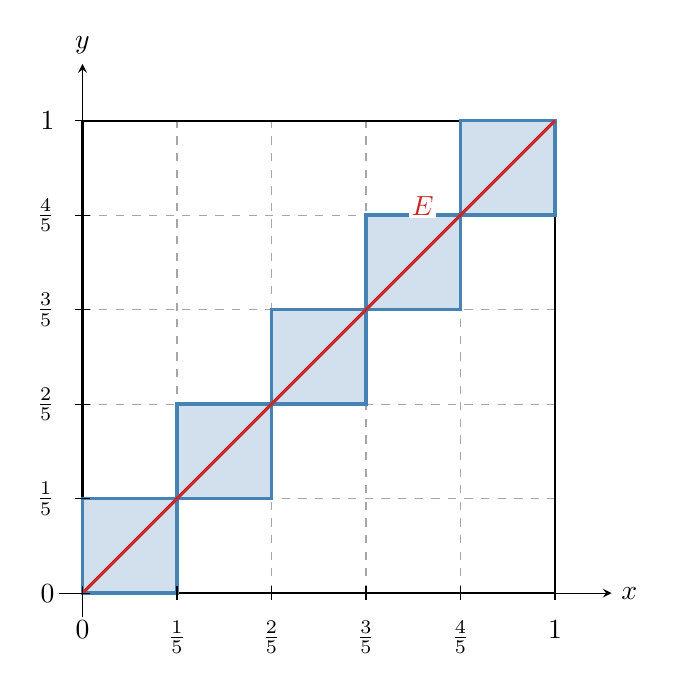
\begin{tikzpicture}[x=6cm,y=6cm,>=stealth]
            \definecolor{qfive}{RGB}{70,130,180}
            \definecolor{ediag}{RGB}{200,40,40}
            \draw[->] (-0.05,0) -- (1.12,0) node[right] {$x$};
            \draw[->] (0,-0.05) -- (0,1.12) node[above] {$y$};
            \fill[qfive!25] (0,0) rectangle (0.2,0.2);
            \fill[qfive!25] (0.2,0.2) rectangle (0.4,0.4);
            \fill[qfive!25] (0.4,0.4) rectangle (0.6,0.6);
            \fill[qfive!25] (0.6,0.6) rectangle (0.8,0.8);
            \fill[qfive!25] (0.8,0.8) rectangle (1,1);
            \draw[step=0.2,gray!70,dashed] (0,0) grid (1,1);
            \draw[thick] (0,0) rectangle (1,1);
            \draw[very thick,qfive] (0,0) rectangle (0.2,0.2);
            \draw[very thick,qfive] (0.2,0.2) rectangle (0.4,0.4);
            \draw[very thick,qfive] (0.4,0.4) rectangle (0.6,0.6);
            \draw[very thick,qfive] (0.6,0.6) rectangle (0.8,0.8);
            \draw[very thick,qfive] (0.8,0.8) rectangle (1,1);
            \draw[very thick,ediag] (0,0) -- (1,1);
            \foreach \k/\lab in {0/0,0.2/\frac15,0.4/\frac25,0.6/\frac35,0.8/\frac45,1/1}{
                \draw (\k,0.015) -- (\k,-0.015) node[below=4pt] {$\lab$};
                \draw (0.015,\k) -- (-0.015,\k) node[left=4pt] {$\lab$};
            }
            \node[ediag,fill=white,inner sep=1pt] at (0.72,0.82) {$E$};
        \end{tikzpicture}
    \end{center}
    For \(y\in[0,1]\), the section \(E^y\) is a singleton and
    \(\mu(E^y)=0\); outside that interval it is empty. For
    \(x\in[0,1]\), \(E_x\) is a singleton and \(\lambda(E_x)=1\).
    Consequently,
    \[
        \int_Y\mu(E^y)\,d\lambda(y)=0,
        \qquad
        \int_X\lambda(E_x)\,d\mu(x)=1.
    \]
    Counting measure on the uncountable space \(Y\) is not
    \(\sigma\)-finite.
\end{snippetexample}

\end{document}
